\documentclass[dvipdfmx,uplatex]{jsarticle}
\def\vector#1{\mbox{\boldmath $#1$}}
\usepackage{qexam} % 問題を書く時とかに必要なやつ
\usepackage{setspace} % 行間開けるのに必要なやつ
\usepackage{amsmath} % 数学やるのに必要なやつ
\usepackage{bm} % 太字にするのに必要なやつ
\usepackage{amssymb}
% 画像を取り込むときに必要なやつ
\usepackage[dvipdfmx]{graphicx}
%\begin{figure}[htbp]
%\begin{center}
%\includegraphics[width=10cm]{フルパス}
%\caption{浜辺美波}
%\end{center}
%\end{figure}

\usepackage{ascmac}
\usepackage{siunitx}
\usepackage{float}
\usepackage{tikz}
\usepackage{circuitikz}
\usepackage{url}
\usepackage{braket}
\usepackage[colorlinks=true, bookmarks=true,
bookmarksnumbered = true, bookmarkstype = toc, linkcolor = black,
urlcolor=black, citecolor=black]{hyperref}
\usepackage{listings,jvlisting} % 日本語のコメントアウトをする場合jvlisting(もしくはjlisting)が必要
\lstset{
  basicstyle={\ttfamily},
  identifierstyle={\small},
  commentstyle={\smallitshape},
  keywordstyle={\small\bfseries},
  ndkeywordstyle={\small},
  stringstyle={\small\ttfamily},
  frame={tb},
  breaklines=true,
  columns=[l]{fullflexible},
  numbers=left,
  xrightmargin=0zw,
  xleftmargin=3zw,
  numberstyle={\scriptsize},
  stepnumber=1,
  numbersep=1zw,
  lineskip=-0.5ex
}%ここまでがプログラムのソースコードを貼るのに必要なやつ
\makeatletter
 \renewcommand{\theequation}{
   \thesubsection.\arabic{equation}}
  \@addtoreset{equation}{subsection}
\title{パターン認識 レポート1}
\author{1019163 日置竜輔 \thanks{公立はこだて未来大学 システム情報科学部 複雑系知能学科 複雑系コース B3}}
\date{\today}

\begin{document}
\begin{spacing}{1.4}

\maketitle
\tableofcontents %目次

\newpage

\section{はじめに}
今回のレポートの最終目標は顔画像に対して、DCT(Discrete Cosine Transformation)係数を求めることであるが、これを行うに当たって、画像処理の知識やDCTの求め方などを知らなかったため、まずはこれらの勉強から始めた。 \\

\subsection{画像処理の基本について学習する}
先ほど述べたようにまずは画像処理をコーディングするための基礎知識として\href{https://github.com/yoyoyo-yo/Gasyori100knock}{画像処理100本ノック!!}というもので知識を深めた。今回はモジュールが豊富という観点からPythonを使用することにした。 \\
ここでは、主に画像処理を行うために必須となる matplotlib, opencv, numpy, skimage などの使い方を勉強した。このノックを行ったことによってある程度画像処理の行い方を学習することができた。

\subsection{DCTとは何か}
画像処理の基本が分かった所で次は課題となっているDCT(以下、離散コサイン変換と呼ぶ)について具体的に調べた。 \\
離散コサイン変換とは、離散信号を周波数領域へ変換する方法の一つであり、信号圧縮に広く用いられている。 \\
離散コサイン変換は、有限数列を、余弦関数数列 $\cos(nk)$ を基底とする一次結合(つまり、適切な周波数と振幅のコサインカーブの和)の係数に変換する。余弦関数は実数に対しては実数を返すので、実数列に対してはDCT係数も実数列となる。\\
離散コサイン変換とよく区別されるのが離散フーリエ変換(DFT: discrete Fourier transform)である。離散フーリエ変換は、実数に対しても複素数を返す$\exp(ink)$ を使用するが、DCTは実数であれば、複素数ではなく実数で返すのが大きな特徴となっている。 \\
離散コサイン変換では、係数が実数になる上、特定の成分への集中度があがるため、JPEGなどの画像圧縮、AACやMP3、ATRACといった音声圧縮、デジタルフィルタ等広い範囲で用いられている。

\subsection{DCTを数学的に理解する}
離散コサイン変換の数学的な具体的な定義は以下のように定められている。\\
\begin{eqnarray*}
0 &\leqq& u, v < T
\end{eqnarray*}
\begin{eqnarray}
F(u, v) &=& \frac{2}{T}C(u)C(v)\sum_{y=0}^{T-1}\sum_{x=0}^{T-1}I(x, y)(\cos\frac{(2x + 1)u\pi}{2T})\cos(\frac{(2y + 1)v\pi}{2T})
\end{eqnarray}

\[\displaystyle
C(u) =
\begin{cases}
\frac{1}{\sqrt{2}} & \quad u = 0 \\
1 & \quad u \neq 0
\end{cases}
\]

このような定義が分かった所で次は実際にPythonでコーディングを行う。

\newpage

\section{プログラムによる実装}
顔画像のDCT係数を計算するに当たって、今回は女優として活躍されている浜辺美波さんの顔画像のDCT係数を求めることにした。

\begin{figure}[htbp]
\begin{center}
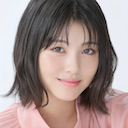
\includegraphics[width=4cm]{/Users/ryusuke/Documents/git/tex/PatternRecognition/Report1/img/minai.png}
\caption{今回使用する浜辺美波の顔画像}
\end{center}
\end{figure}

\subsection{pythonによる実装}

\begin{lstlisting}[caption=DCT係数を求めるソースコード]
# DCT hyoer-parameter
img_128 = io.imread("img/hamabe-minai.png")

# DCT
def dct(img, T=8, channel=3):
    H, W, _ = img.shape
    F = np.zeros((H, W, channel), dtype=np.float32)

    theta = np.pi / (2 * T)

    for c in range(channel):
        for vi in range(0, H, T):
            for ui in range(0, W, T):
                for v in range(T):
                    for u in range(T):
                        cu = 1 / np.sqrt(2) if u == 0 else 1
                        cv = 1 / np.sqrt(2) if v == 0 else 1
                        coef1, coef2 = np.meshgrid(np.cos((2 * np.arange(0, T) + 1) * u * theta), np.cos((2 * np.arange(0, T) + 1) * v * theta))
                        F[vi + v, ui + u, c] = 2 * cu * cv * np.sum(img[vi : vi + T, ui : ui + T, c] * coef1 * coef2) / T
    return F

# DCT
F = dct(img_128) # 画像に対してDCT係数を求める

\end{lstlisting}

\subsection{DCT係数を出力する}
2.1で求めたFに128*128画素の3次元ベクトルが格納されているので、これを出力することでDCT係数を得ることができる。

\begin{lstlisting}[caption=DCT係数を出力するソースコード]
with open('output.txt', 'w') as f: # outputという名前のテキストファイルを作成する
    for y in range(len(F)): # 縦の128画素
        for x in range(len(F[y])): # 横の128画素
            f.write(str(y) + " " + str(x) + "\n") # (y, x) の座標を書き込む
            f.write(str(F[y][x]) + "n") # 3次元ベクトルを書き込む
\end{lstlisting}

上記のコードで得られた係数のサンプルが下図である。\\
2つの数字は2次元ユークリッド座標 $(y, x)$ を表しており、続く3つの配列は成分のベクトルを表している。\\
.txtの拡張子で保存するにはstr型で保存する必要があるので、listで受け取った配列をstrに戻して入力する実装を行う。
\begin{figure}[htbp]
\begin{center}
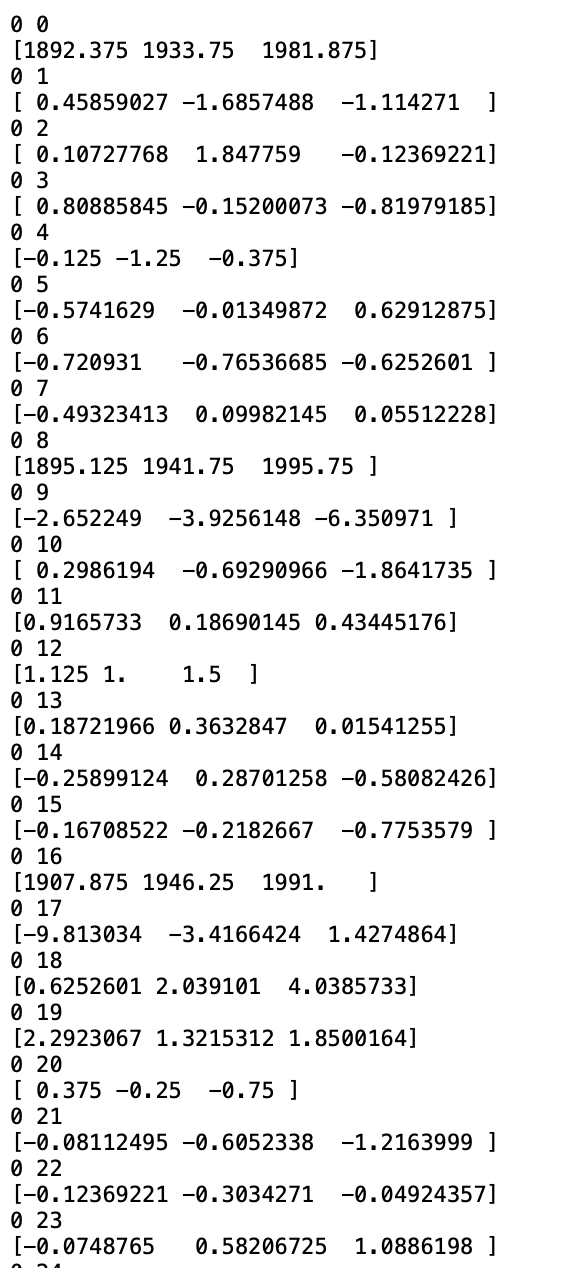
\includegraphics[width=5cm]{/Users/ryusuke/Documents/git/tex/PatternRecognition/Report1/output/output_example_1.png}
\caption{DCT係数の出力結果の一部分}
\end{center}
\end{figure}

\newpage

\section{逆離散コサイン変換を行う}
第2章で離散コサイン変換を行い、DCT係数を求める作業を行った。そして、課題とはなっていないが、これらの数値から元の画像に復元できないかと思い、実装してみることにした。
\subsection{逆離散コサイン変換}
逆離散コサイン変換(IDCT: Inverse Discrete Cosine Transformation)とは離散コサイン変換の逆(復号)であり、次式で定義される。ここでいう K は復元時にどれだけ解像度を良くするかを決定するパラメータである。\\
K = Tの時は、DCT係数を全部使うのでIDCT後の解像度は最大になるが、Kが1や2などの時は復元に使う情報量(DCT係数)が減るので解像度が下がる。これを適度に設定することで、画像の容量を減らすことができる。\\

IDCTは数学的には以下のように定義されている。
\begin{eqnarray*}
1 &\leqq& K \leqq T
\end{eqnarray*}
\begin{eqnarray}
F(x, y) &=& \frac{2}{T}\sum_{y=0}^{T-1}\sum_{x=0}^{T-1}C(u)C(v)F(u, v)(\cos\frac{(2x + 1)u\pi}{2T})\cos(\frac{(2y + 1)v\pi}{2T})
\end{eqnarray}
\[\displaystyle
C(u) =
\begin{cases}
\frac{1}{\sqrt{2}} & \quad u = 0 \\
1 & \quad u \neq 0
\end{cases}
\]

上記のように定められているため、これを用いて画像の復元を行う。

\subsection{IDCTを用いて顔画像の復元}
コードは下記のようなものになった。
\begin{lstlisting}[caption=DCT係数を元に画像を復元するソースコード]
# DCT hyoer-parameter
img_128 = io.imread("img/hamabe-minai.png")

# DCT
def dct(img, T=8, channel=3):
    H, W, _ = img.shape
    F = np.zeros((H, W, channel), dtype=np.float32)

    theta = np.pi / (2 * T)

    for c in range(channel):
        for vi in range(0, H, T):
            for ui in range(0, W, T):
                for v in range(T):
                    for u in range(T):
                        cu = 1 / np.sqrt(2) if u == 0 else 1
                        cv = 1 / np.sqrt(2) if v == 0 else 1
                        coef1, coef2 = np.meshgrid(np.cos((2 * np.arange(0, T) + 1) * u * theta), np.cos((2 * np.arange(0, T) + 1) * v * theta))
                        F[vi + v, ui + u, c] = 2 * cu * cv * np.sum(img[vi : vi + T, ui : ui + T, c] * coef1 * coef2) / T
    return F

# IDCT
def idct(F,  T=8, K=8, channel=3):
    H, W, _ = F.shape
    out = np.zeros((H, W, channel), dtype=np.float32)

    theta = np.pi / (2 * T)

    c_mat = np.ones([T, T])
    c_mat[0] /= np.sqrt(2)
    c_mat[:, 0] /= np.sqrt(2)
   # print(c_mat)
    for c in range(channel):
        for yi in range(0, H, T):
            for xi in range(0, W, T):
                for y in range(T):
                    for x in range(T):
                        coef1, coef2 = np.meshgrid(np.cos((2 * x + 1) * np.arange(0, T) * theta), np.cos((2 * y + 1) * np.arange(0, T) * theta))
                        out[yi + y, xi + x, c] = 2 * np.sum(F[yi : yi + K, xi : xi + K, c] * coef1[:K, :K] * coef2[:K, :K] * c_mat[:K, :K]) / T

    out = np.clip(out, 0, 255)
    out = np.round(out).astype(np.uint8)

    return out

# DCT
F = dct(img_128) # DCT係数を求める

# IDCT
out = idct(F) # DCT係数を用いて顔画像を復元する

plt.figure(figsize=(12, 4))
plt.subplot(1, 2, 1)
plt.title("Original")
plt.imshow(img_128)

plt.subplot(1, 2 ,2)
plt.title("Face image after using IDCT")
plt.imshow(out)
plt.show()
\end{lstlisting}

上記のコードを実行して得られた結果が以下のようになる。\\
\begin{figure}[htbp]
\begin{center}
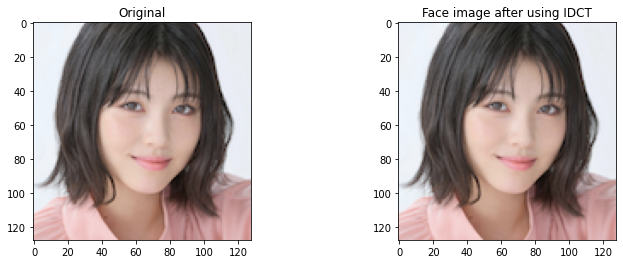
\includegraphics[width=10cm]{/Users/ryusuke/Documents/git/tex/PatternRecognition/Report1/output/output.png}
\caption{DCT係数を用いて復元した後の浜辺美波の顔画像}
\end{center}
\end{figure}

得られた画像の方が色合いが少し濃くなっていることがわかるが、顔の形や色はかなり再現されていることが確認できる。
\newpage

\section{最後に}
今回は指定された顔画像のDCT係数を求めるということだけでなく、さらにIDCTを用いて顔画像の復元を行うということまで実装した。結果的にほとんど元の画像と一致して結果が得られたので安心した。\\
DCTは前述でも述べたように、JPEGなどの画像圧縮、AACやMP3、ATRACといった音声圧縮、デジタルフィルタ等広い範囲で用いられており、画像処理についてはまだまだ知らないことが多くあると感じたので、講義が終わった後も自主的に学んでいきたいと感じた。

\end{spacing}
\end{document}
